\chapter{Evaluation}

\section{Customer Requirements}

Below is a list of all my general and specific objectives that I set myself in the analysis section. In this section I will determine whether I have met all of these objectives and the reasoning behind it. The subsections with *NEW* in the title are objectives that I did not identify in my analysis section; however during the course of my implementation, I attempted to meet the objectives. 

\subsection{Aesthetically pleasing, easy to navigate GUI.} %Need feedback

This objective has been met.




\subsection{Videos organised and filtering capabilities.}

This objective has been partially met. The video links (tricks tutorial link) are organised in the tricks table in the order of TrickID; however there are no fitering capabilities implemented in the program at this stage. 


\begin{figure}[H]
    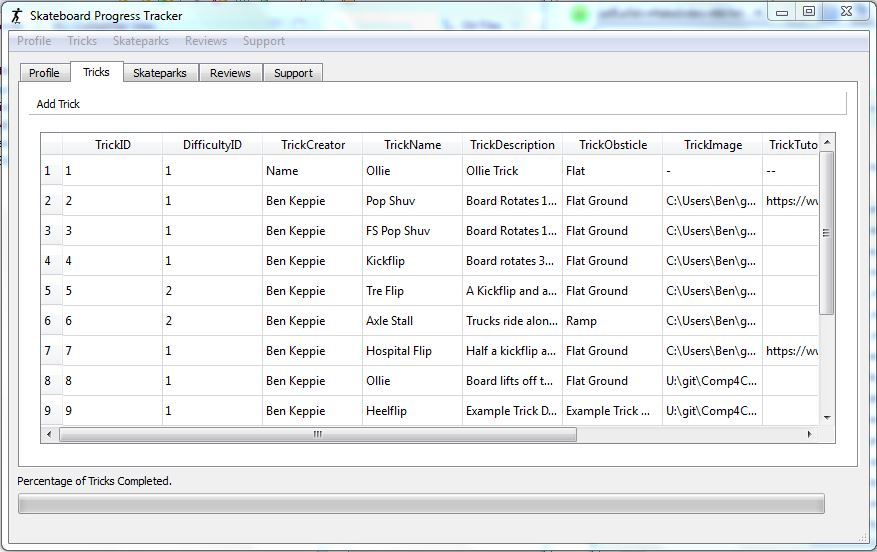
\includegraphics[width=\textwidth]{./Evaluation/images/OrganisedTricks.jpg}
    \caption{Tricks Organised by TrickID} \label{fig:TricksOrganised}
\end{figure}

The figue above shows that the video links have been organised by TrickID. With the first TrickID being at the top of the table and the last being at the bottom; however, from the figure above you can see that there are no filtering capabilities within the Tricks tab which contribute to the functionality of filtering the tricks table.




\subsection{Correct and accurate mapping to the skate parks/spots.}

This objective has not been met.



\subsection {Correct directions from current location to skate park/ spot on the map.}

This objective has not been met.



\subsection{Non-biased reviews.}

This objective has been met to an extent. As the program is currently a single user application, the only reviews that will be in place will be the reviews that my client adds. Therefore the only way the review would be biased is if my client specifically made a biased review. 



\subsection{Clear database with a list of tricks in.} %Need feedback

This objective has been met.


\subsection{ Easy to filter through tricks known.}

This objective has not been met. As discussed before, filtering capabilities have not been implemented in this version of the program.



\subsection {Display status bar messages at appropriate times to inform the user of changes *NEW*} %FEEDBACK

This objective has been met.



\subsection {Allow for the user to contact the developer *NEW*}

This objective has been met.


\begin{figure}[H]
    \includegraphics[width=\textwidth]{./Evaluation/images/Contactsupport.jpg}
    \caption{Contacting Developer Form} \label{fig:ContactSupportEVD}
\end{figure}

The figure above shows the form in the support tab which users can fill in, in order to contact the developer with any problems or queries about the program.



\subsection {Ensure that the profile picture can be changed easily *NEW*} %Need feedback

This objective has been met.



\subsection {Ensure that the profile name can be edited easily *NEW*} %Need feedback

This objective has been met.




\subsection {Ensure that the profile email can be edited easily *NEW*} %Need feedback

This objective has been met.




\subsection {Ensure that videos can be filtered by categories. e.g easy, medium, hard tricks.}

This objective hasn't been met.




\subsection {Ensure that videos load correctly and are linked to the right video.}

This objective has been met. I have used a regular expression to validate an official YouTube video link, and on top of that referential integrity has been enforced in the database so that the tutorial link will be assigned to the trick that it was added to by the user. 




\subsection {Ensure that videos are displayed at the correct size/resolution that the monitor of the computer is.}

This objective hasn't been met.



\subsection {Ensure the database can add, edit and remove trick data (Name, description, image, completed status and tutorial link).}

This objective hasn't been met. However part of the objective has.

\subsection {Ensure that the database is displayed correctly inside the application at all resolutions.}

This objective has been met.

\subsection {Ensure that the tricks are marked by how hard they are by a three way scale of: Easy, Medium or Hard.}

This objective has been met.

\subsection {Ensure a checkbox is by the side of a trick to represent whether the user has completed that trick or not.}

This objective hasn't been met.

\subsection {Ensure there is a search bar for a specific trick name.}

This objective hasn't been met.

\subsection {Ensure there are filters for tricks e.g Switch trick filters.}

This objective hasn't been met.



\subsection {Ensure that the map is accurate to current roads.}

This objective has been met.

\subsection {Ensure location of the user is not revealed to anyone else.}

This objective has been met.

\subsection {Ensure that the current location marker is accurate.}

This objective hasn't been met.

\subsection {Ensure that when giving directions to skate parks from your current location that the mapping route is correct and on viable roads. }

This objective hasn't been met.

\subsection {Ensure that the program can mark skate park locations.}

This objective has been met.


\subsection {Ensure no biased reviews are posted to the app and that they're moderated before they are universally posted.}

This objective has been met.

\subsection {Ensure the program runs fast without lag when navigating between areas of the application.}  %Need Feedback.

This objective has been met.



\section{Effectiveness}

%include as many subsections as necessary for your objectives - Only evaluate the objectives you met
\subsection{Objective Evaluation}

\section{Learnability}

\section{Usability}

\section{Maintainability}

\section{Suggestions for Improvement}

\section{End User Evidence}

\subsection{Questionnaires}

\subsubsection{Client Feedback Questionnaire} %TRIM PDF


\begin{figure}[H]
    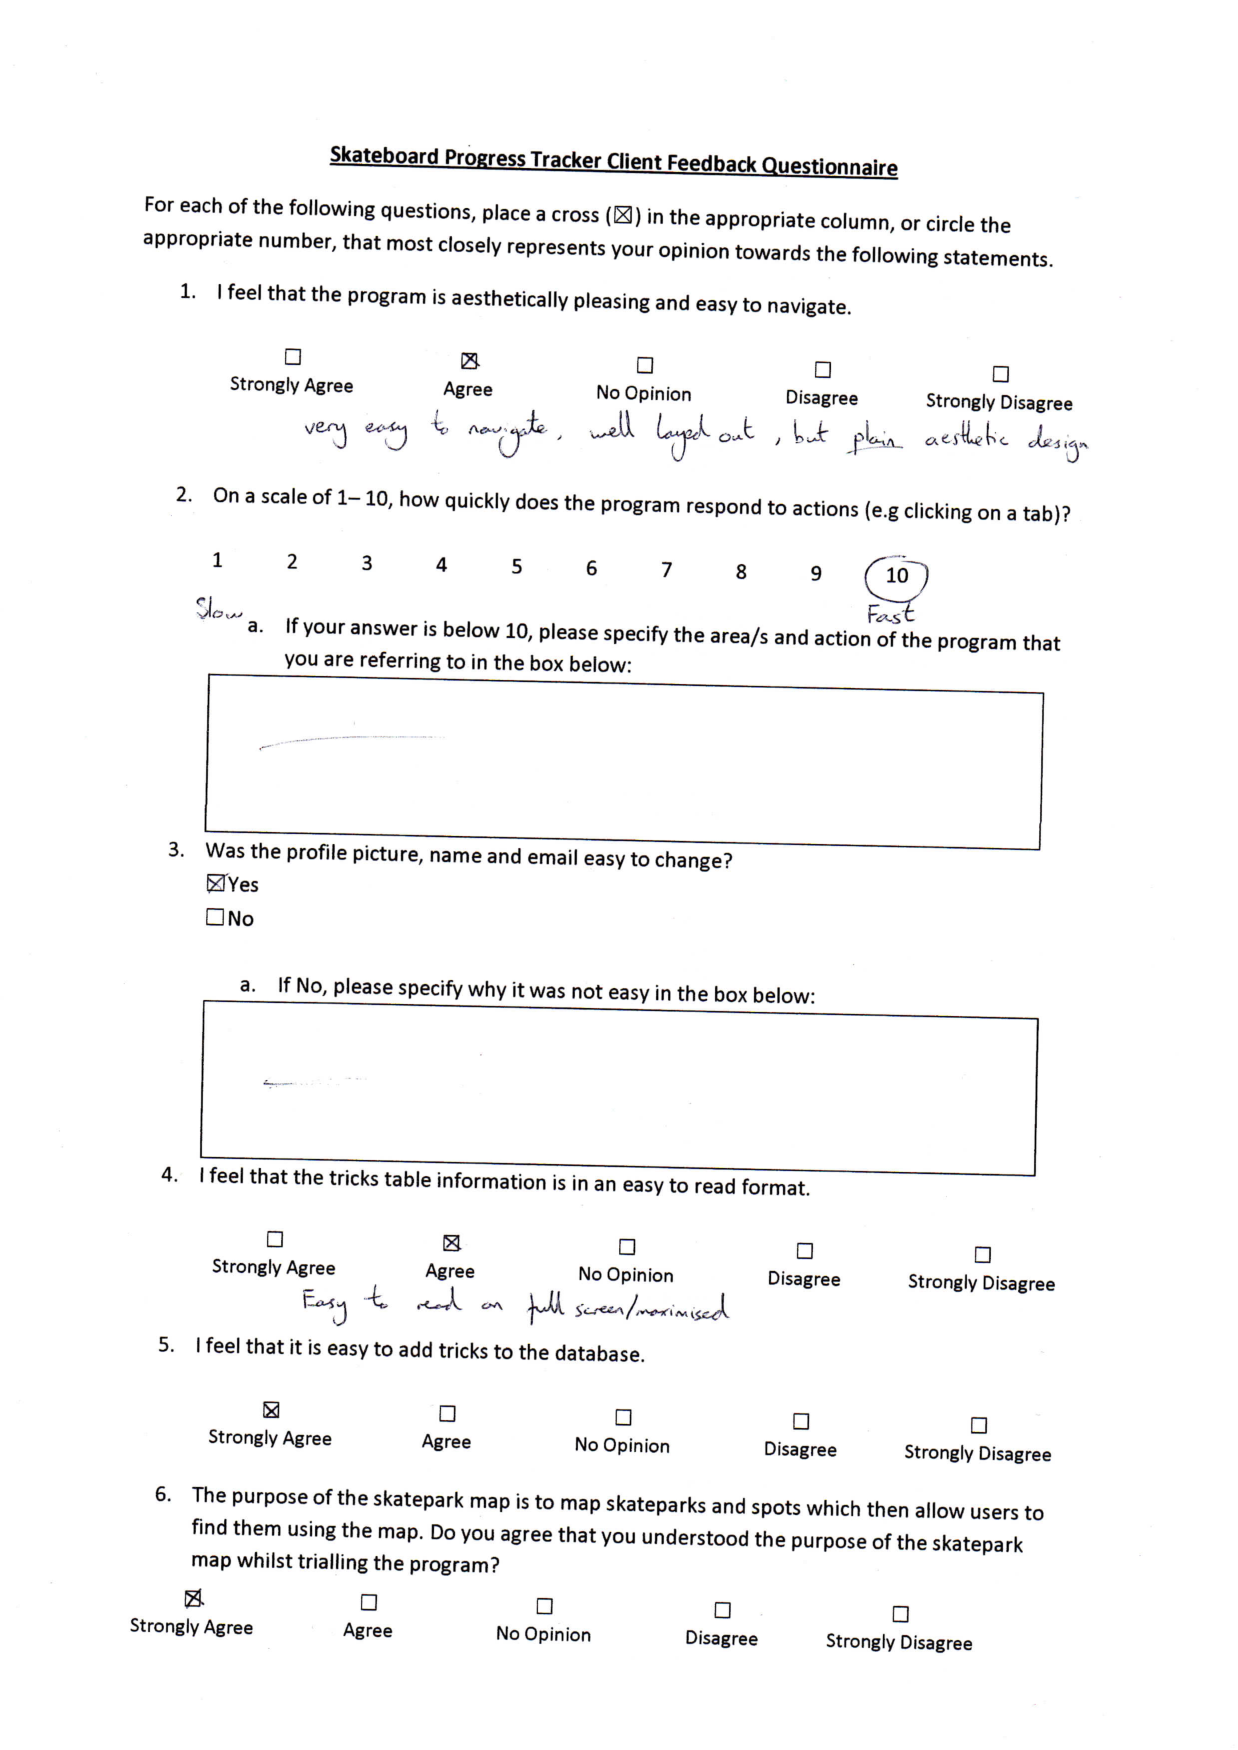
\includegraphics[width=\textwidth]{./Evaluation/images/StuFeedback1.pdf}
    \caption{Stuart Keppie Client Feedback Part 1} \label{fig:StuFeedback1}
\end{figure}

\begin{figure}[H]
    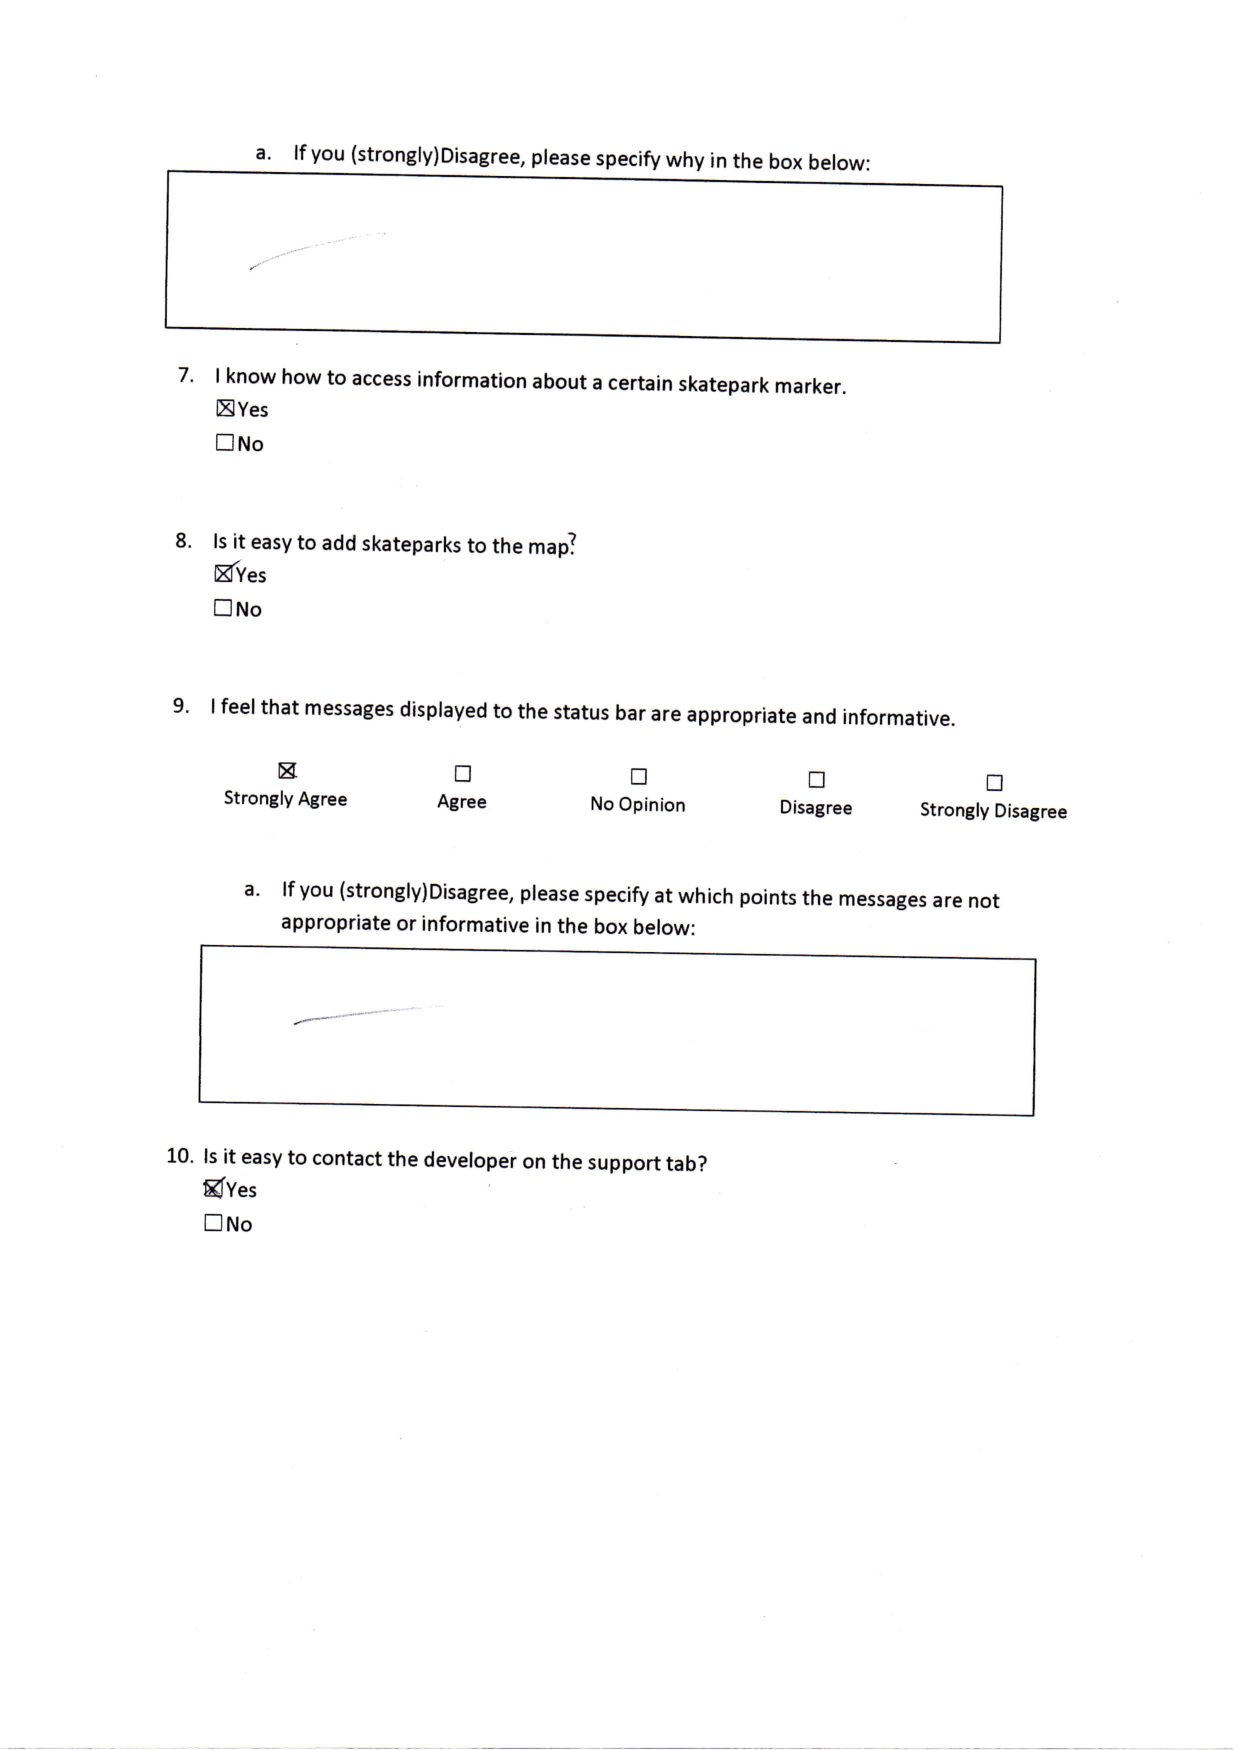
\includegraphics[width=\textwidth]{./Evaluation/images/StuFeedback2.pdf}
    \caption{Stuart Keppie Client Feedback Part 2} \label{fig:StuFeedback2}
\end{figure}

\begin{figure}[H]
    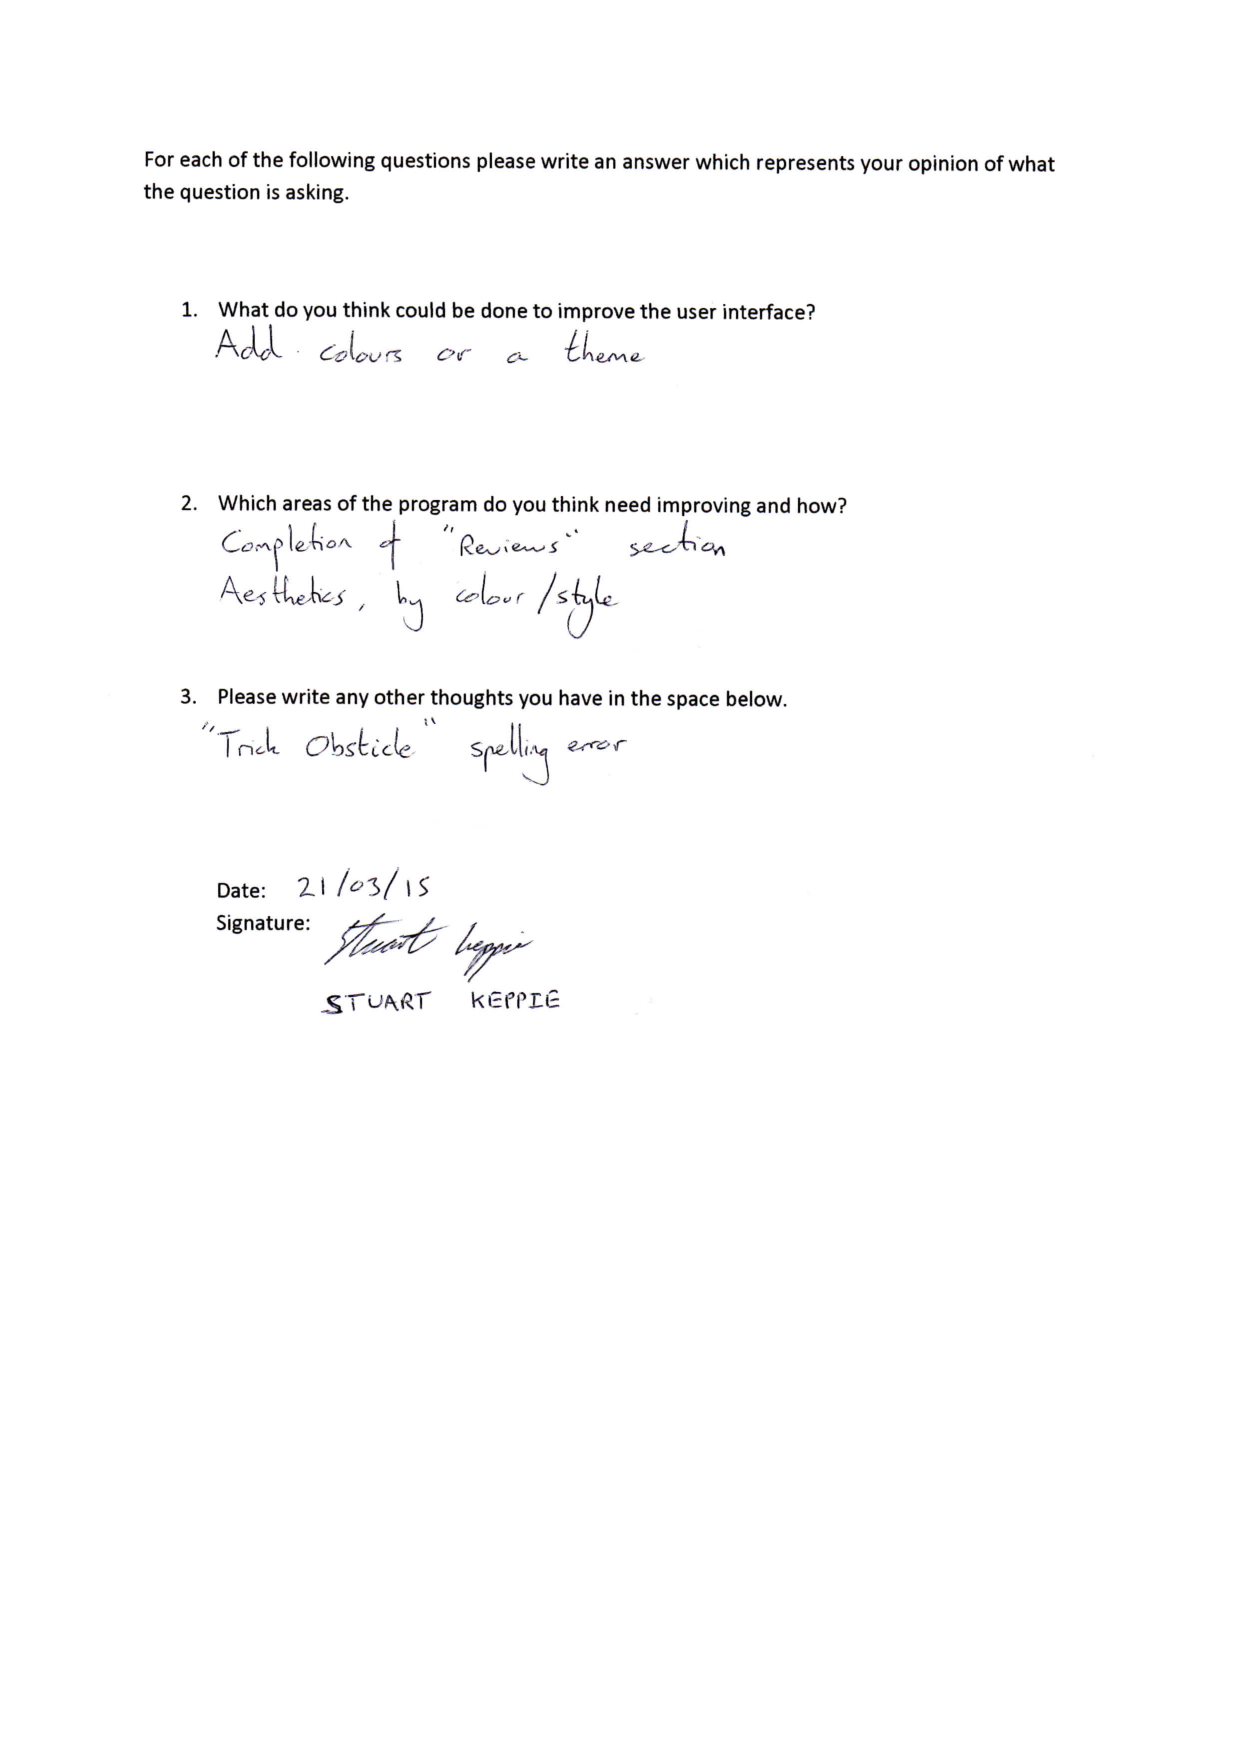
\includegraphics[width=\textwidth]{./Evaluation/images/StuFeedback3.pdf}
    \caption{Stuart Keppie Client Feedback Part 3} \label{fig:StuFeedback3}
\end{figure}

\subsubsection{General Feedback Questionnaire}

\begin{figure}[H]
    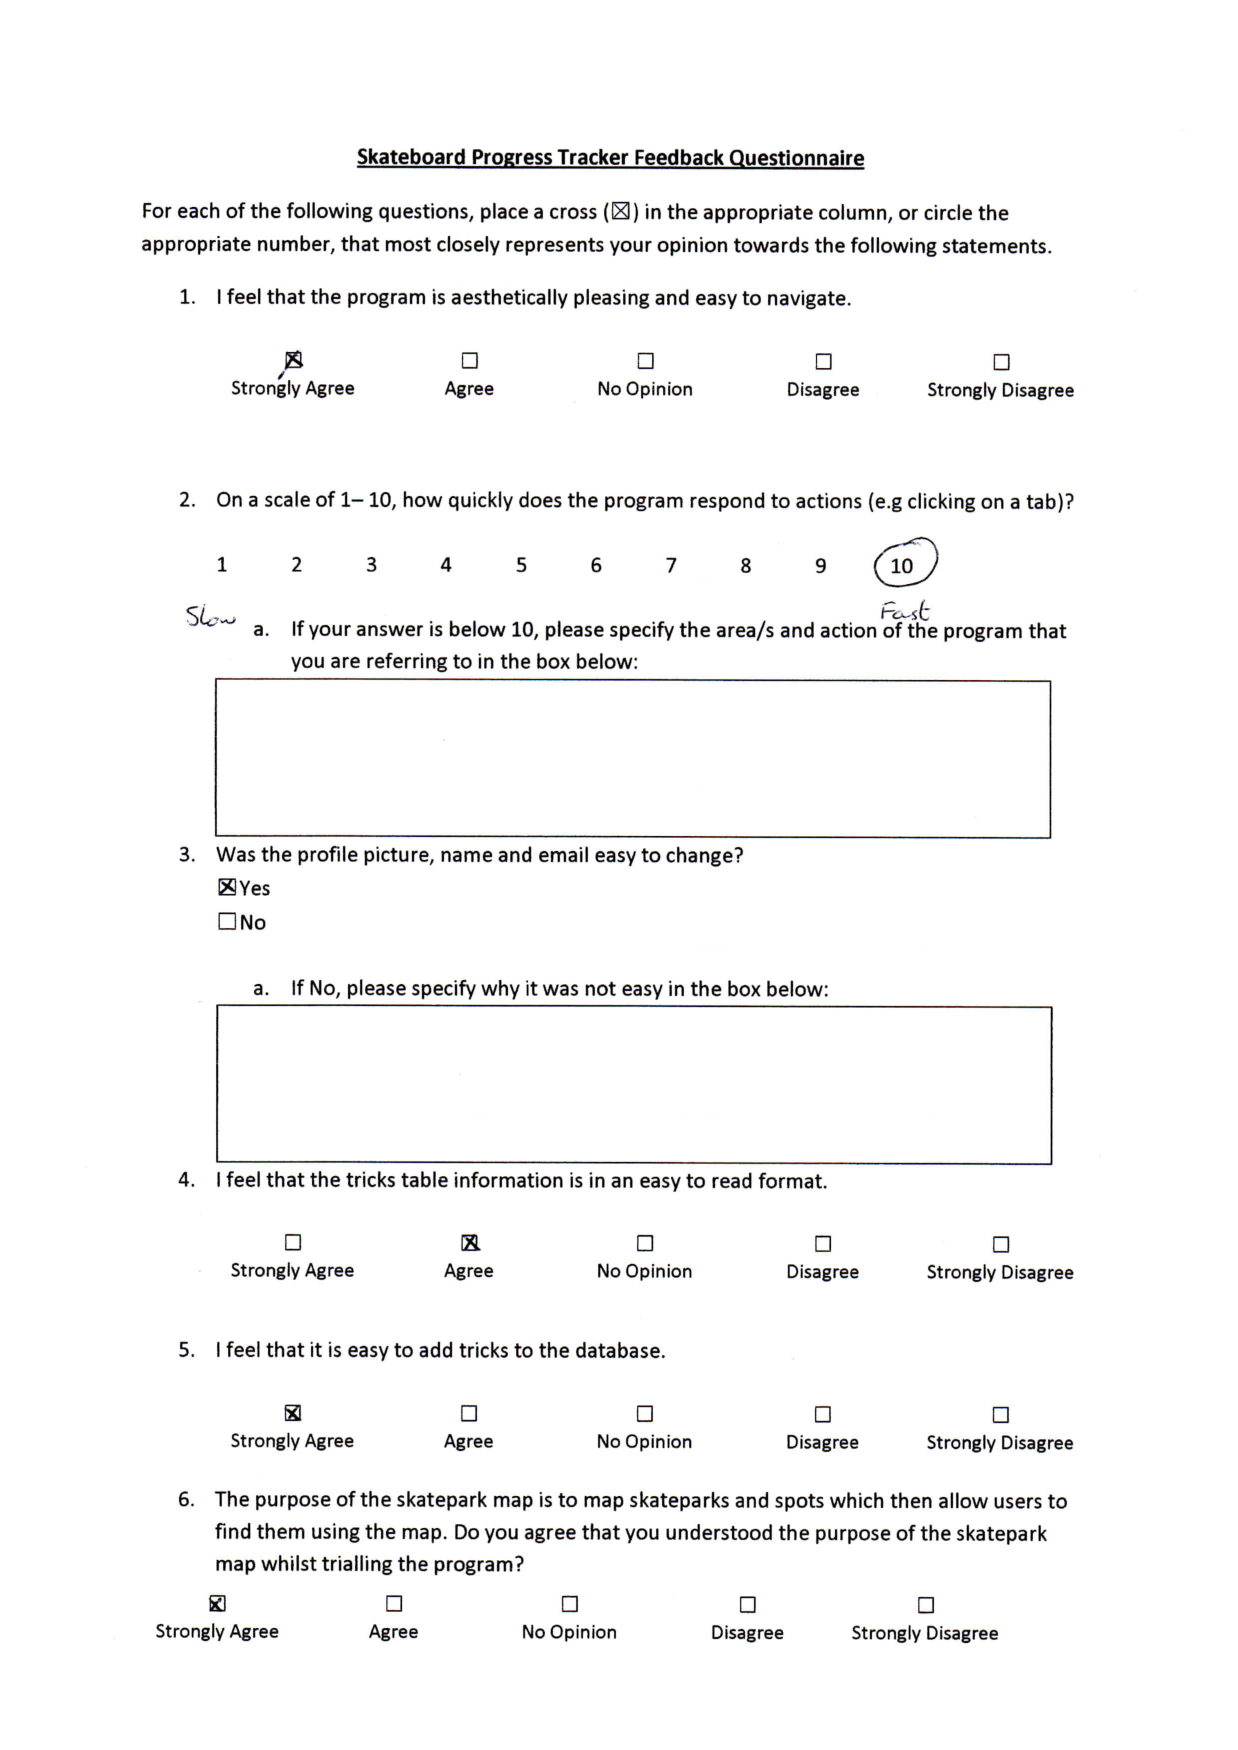
\includegraphics[width=\textwidth]{./Evaluation/images/PierreFeedback1.pdf}
    \caption{Pierre Feedback Part 1} \label{fig:PierreFeedback1}
\end{figure}

\begin{figure}[H]
    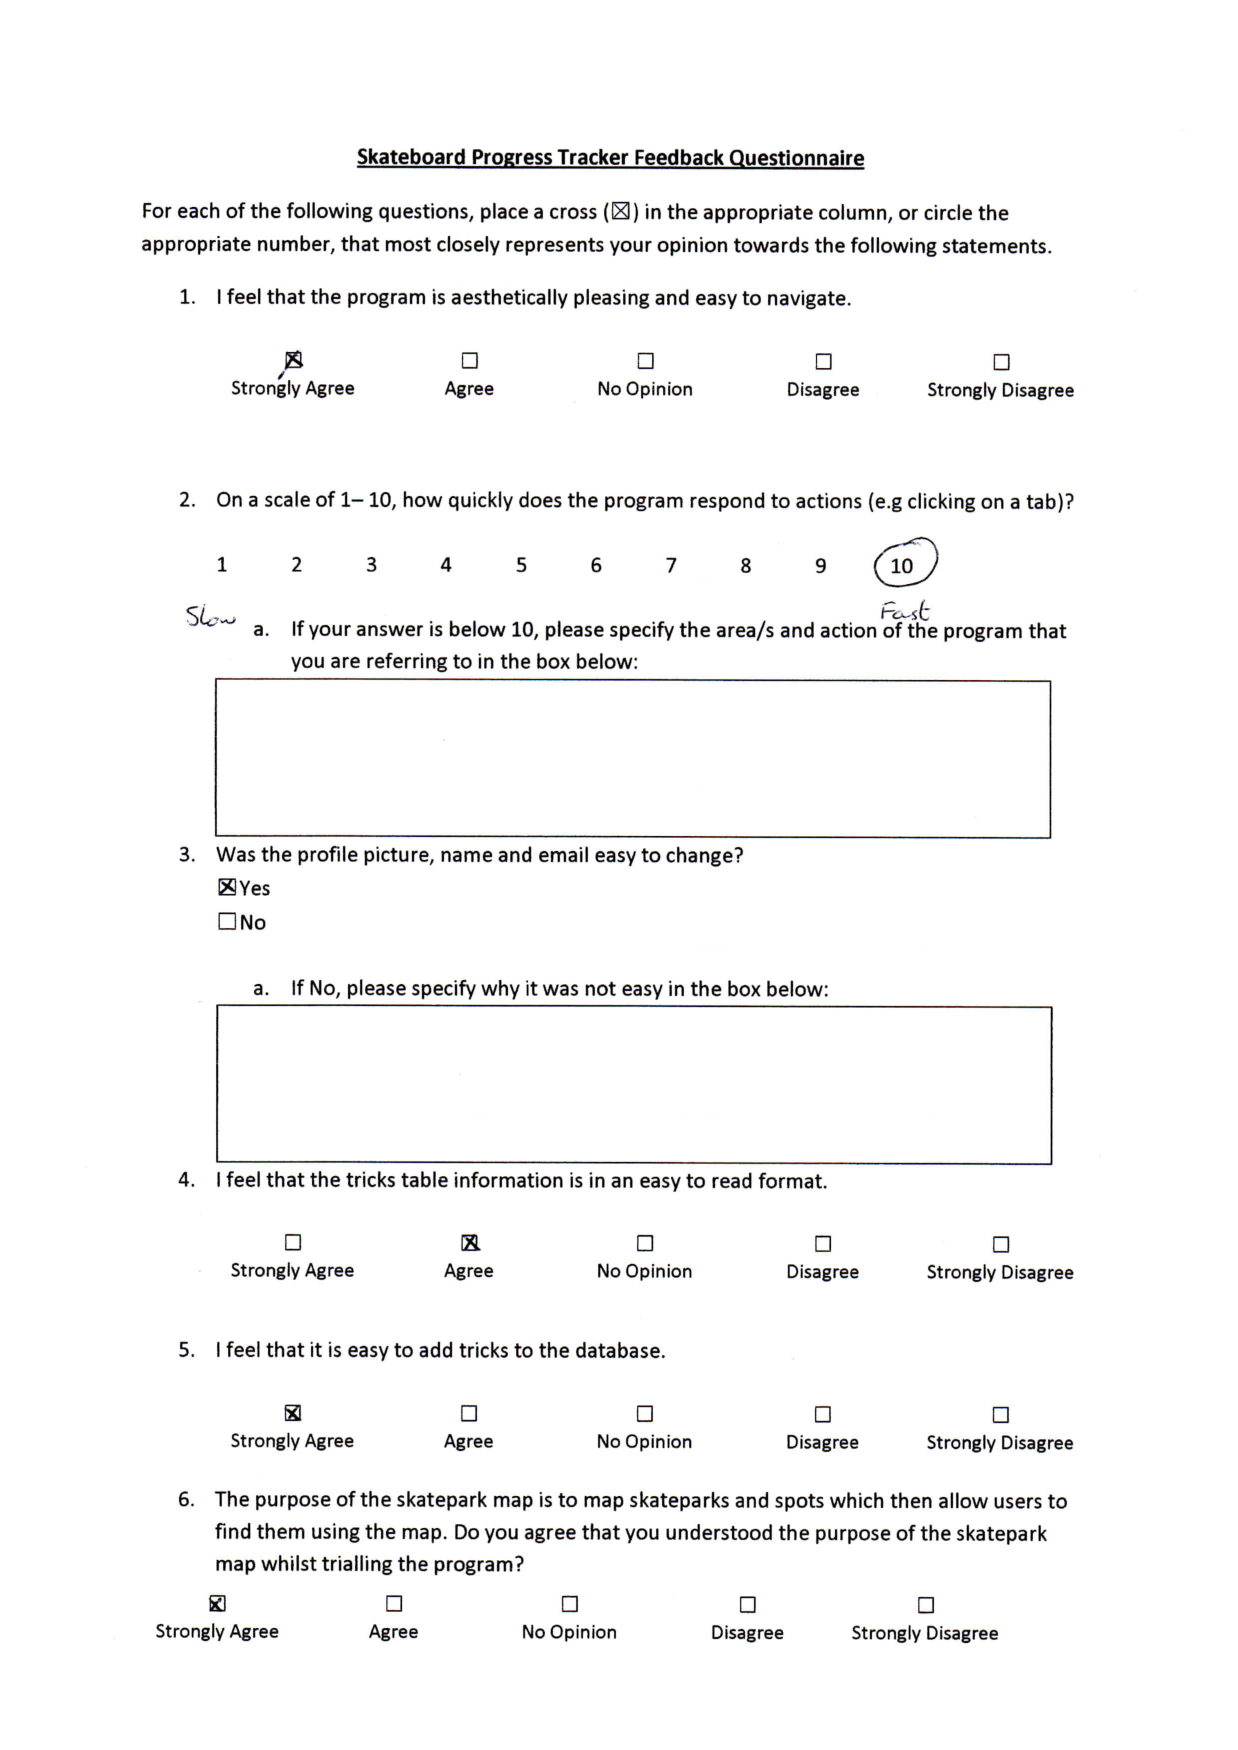
\includegraphics[width=\textwidth]{./Evaluation/images/PierreFeedback1.pdf}
    \caption{Pierre Feedback Part 2} \label{fig:PierreFeedback2}
\end{figure}

\begin{figure}[H]
    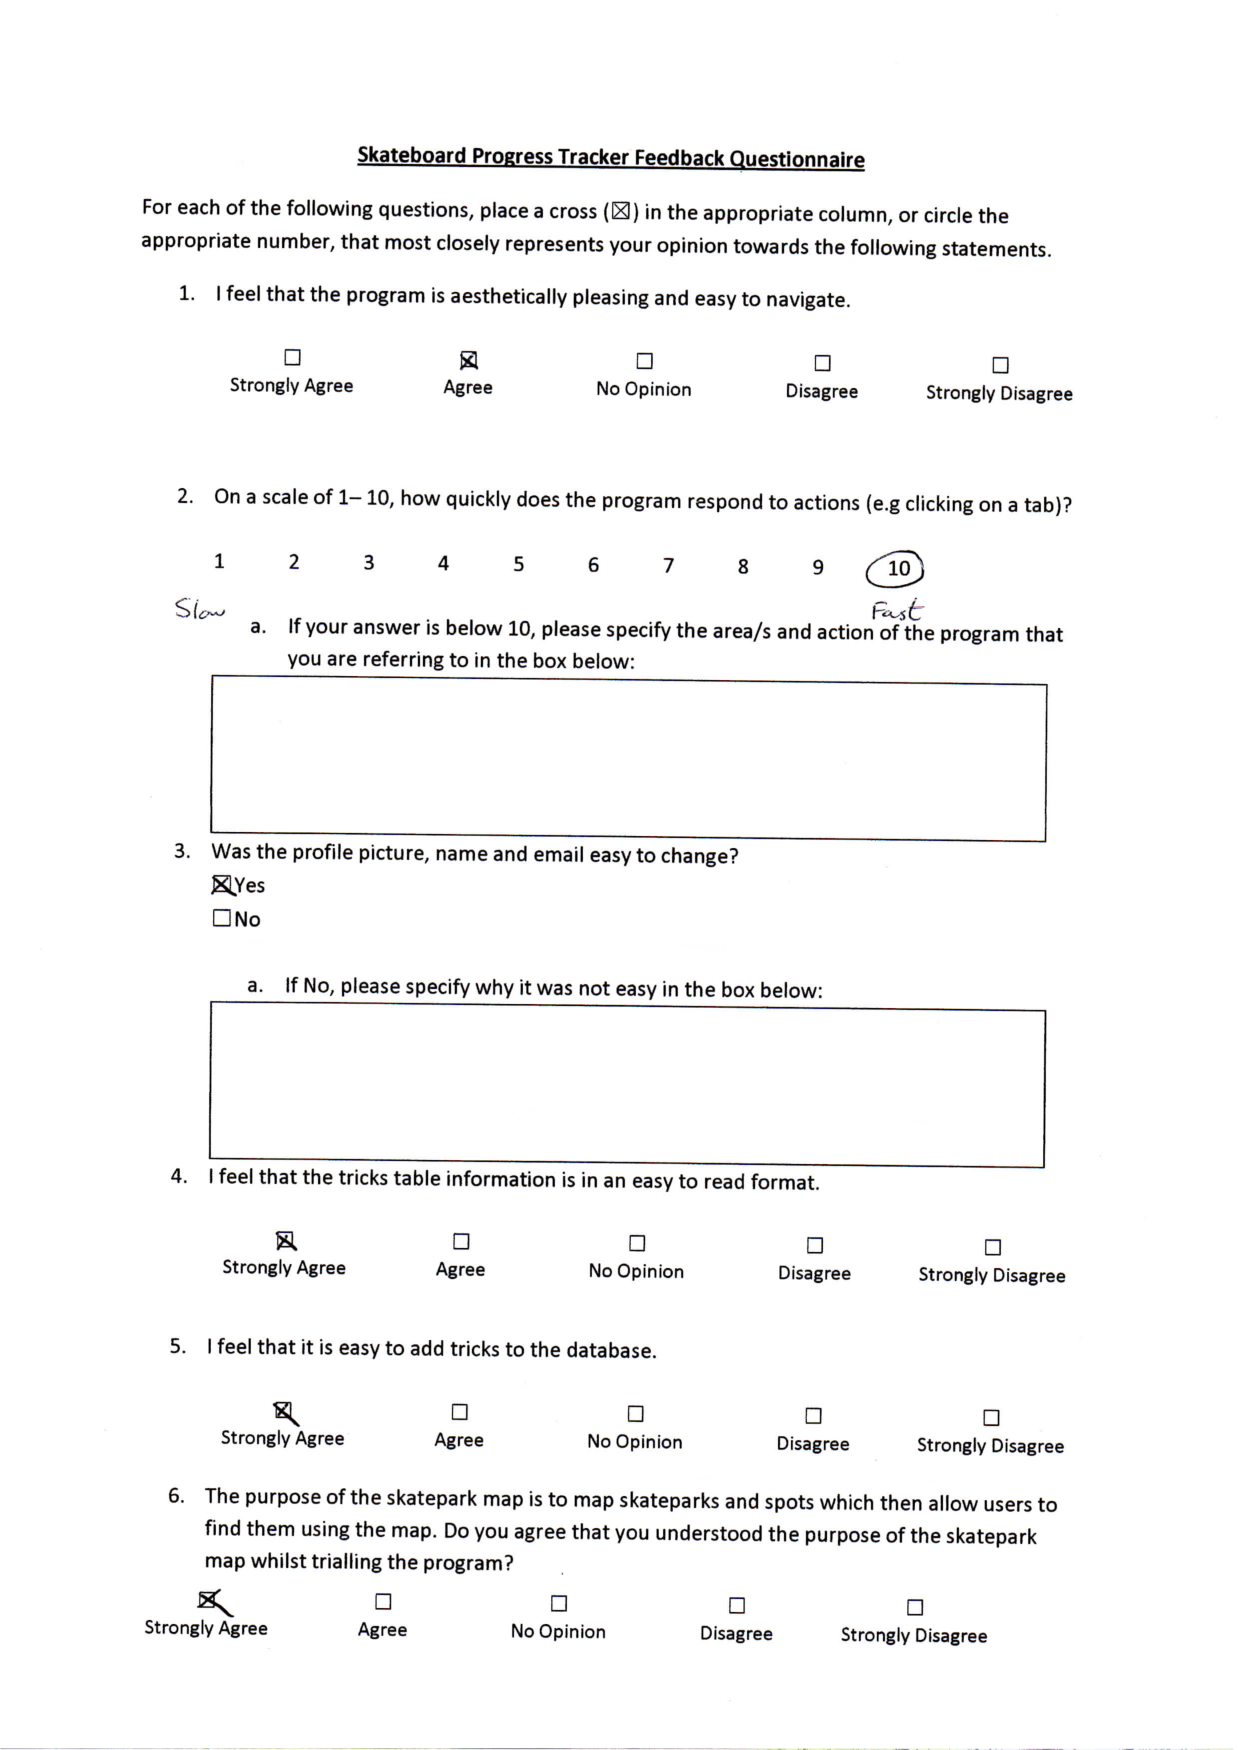
\includegraphics[width=\textwidth]{./Evaluation/images/LeucilleFeedback1.pdf}
    \caption{Leucille Feedback Part 1} \label{fig:LeucilleFeedback1}
\end{figure}

\begin{figure}[H]
    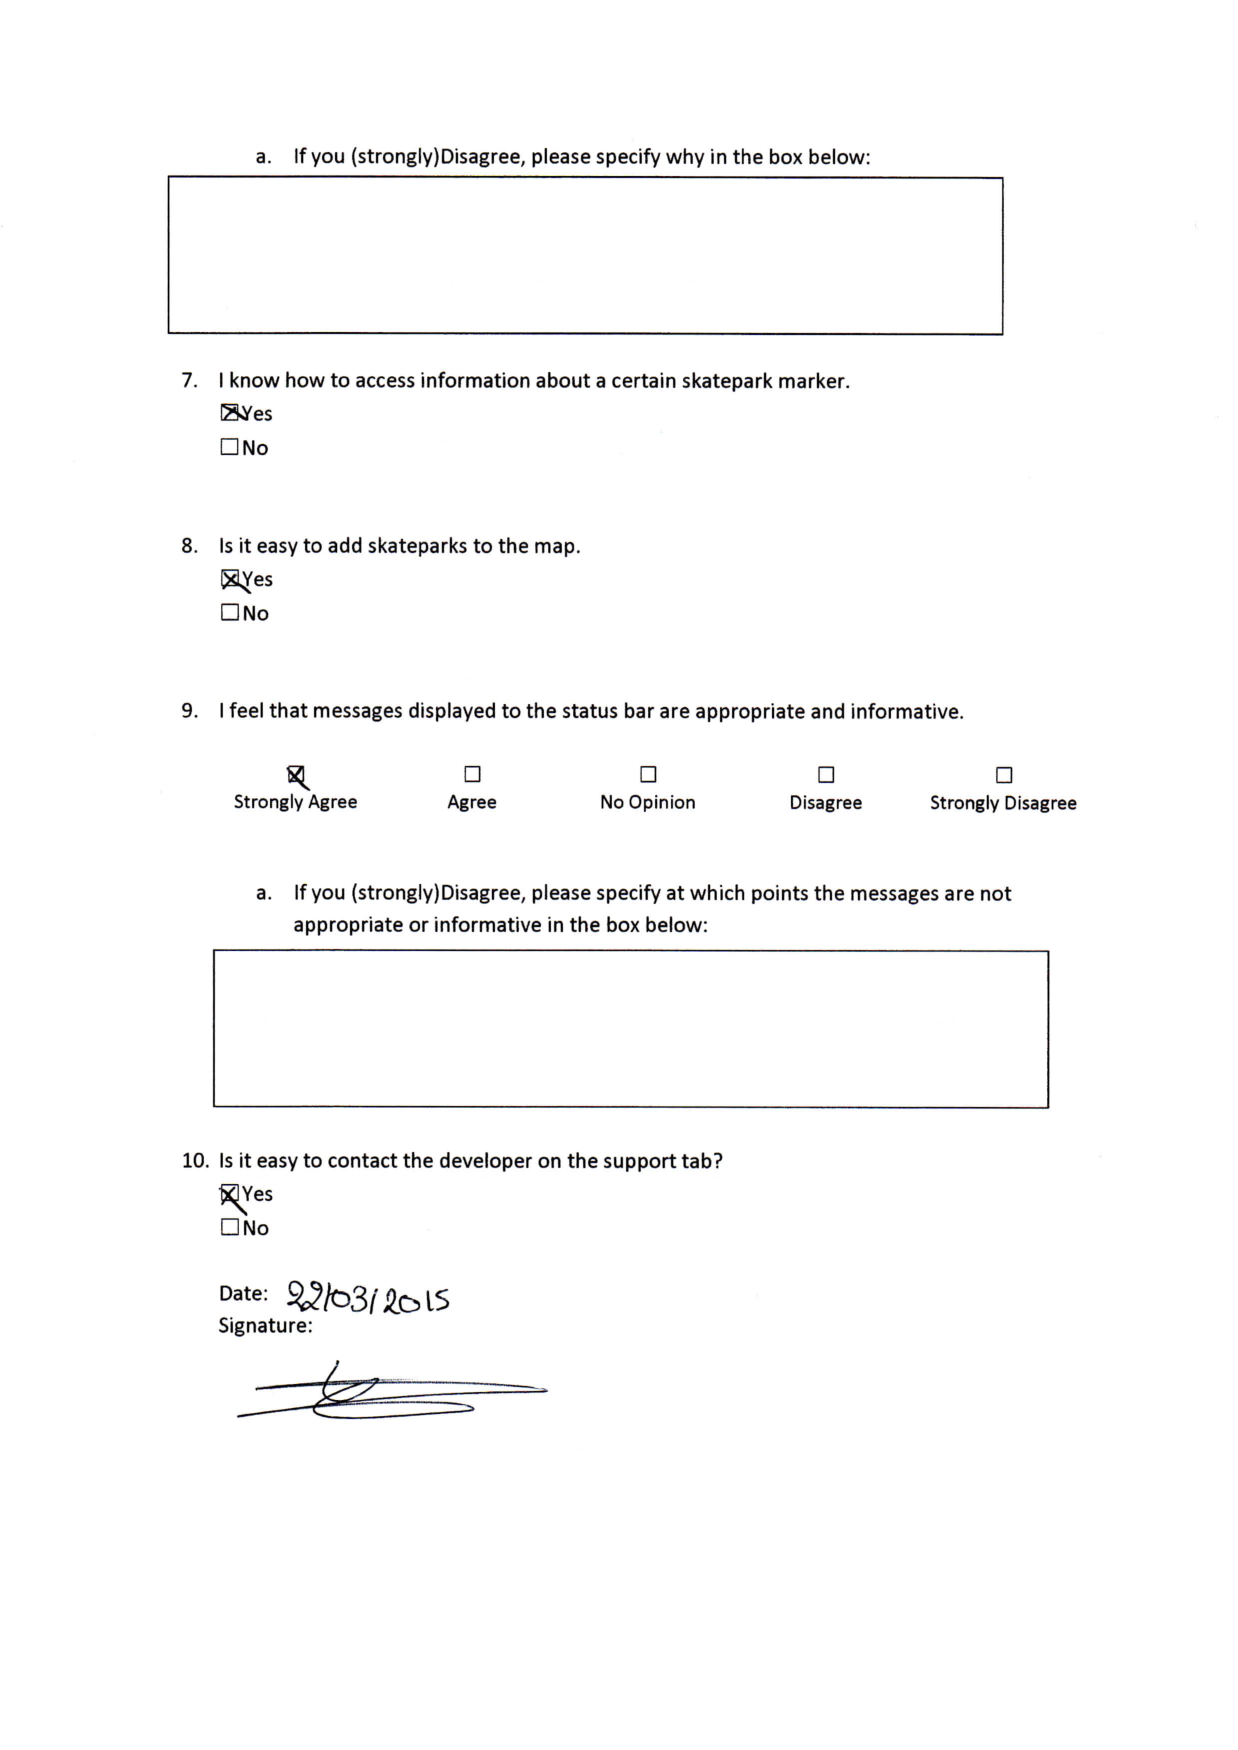
\includegraphics[width=\textwidth]{./Evaluation/images/LeucilleFeedback2.pdf}
    \caption{Leucille Feedback Part 2} \label{fig:LeucilleFeedback2}
\end{figure}

\begin{figure}[H]
    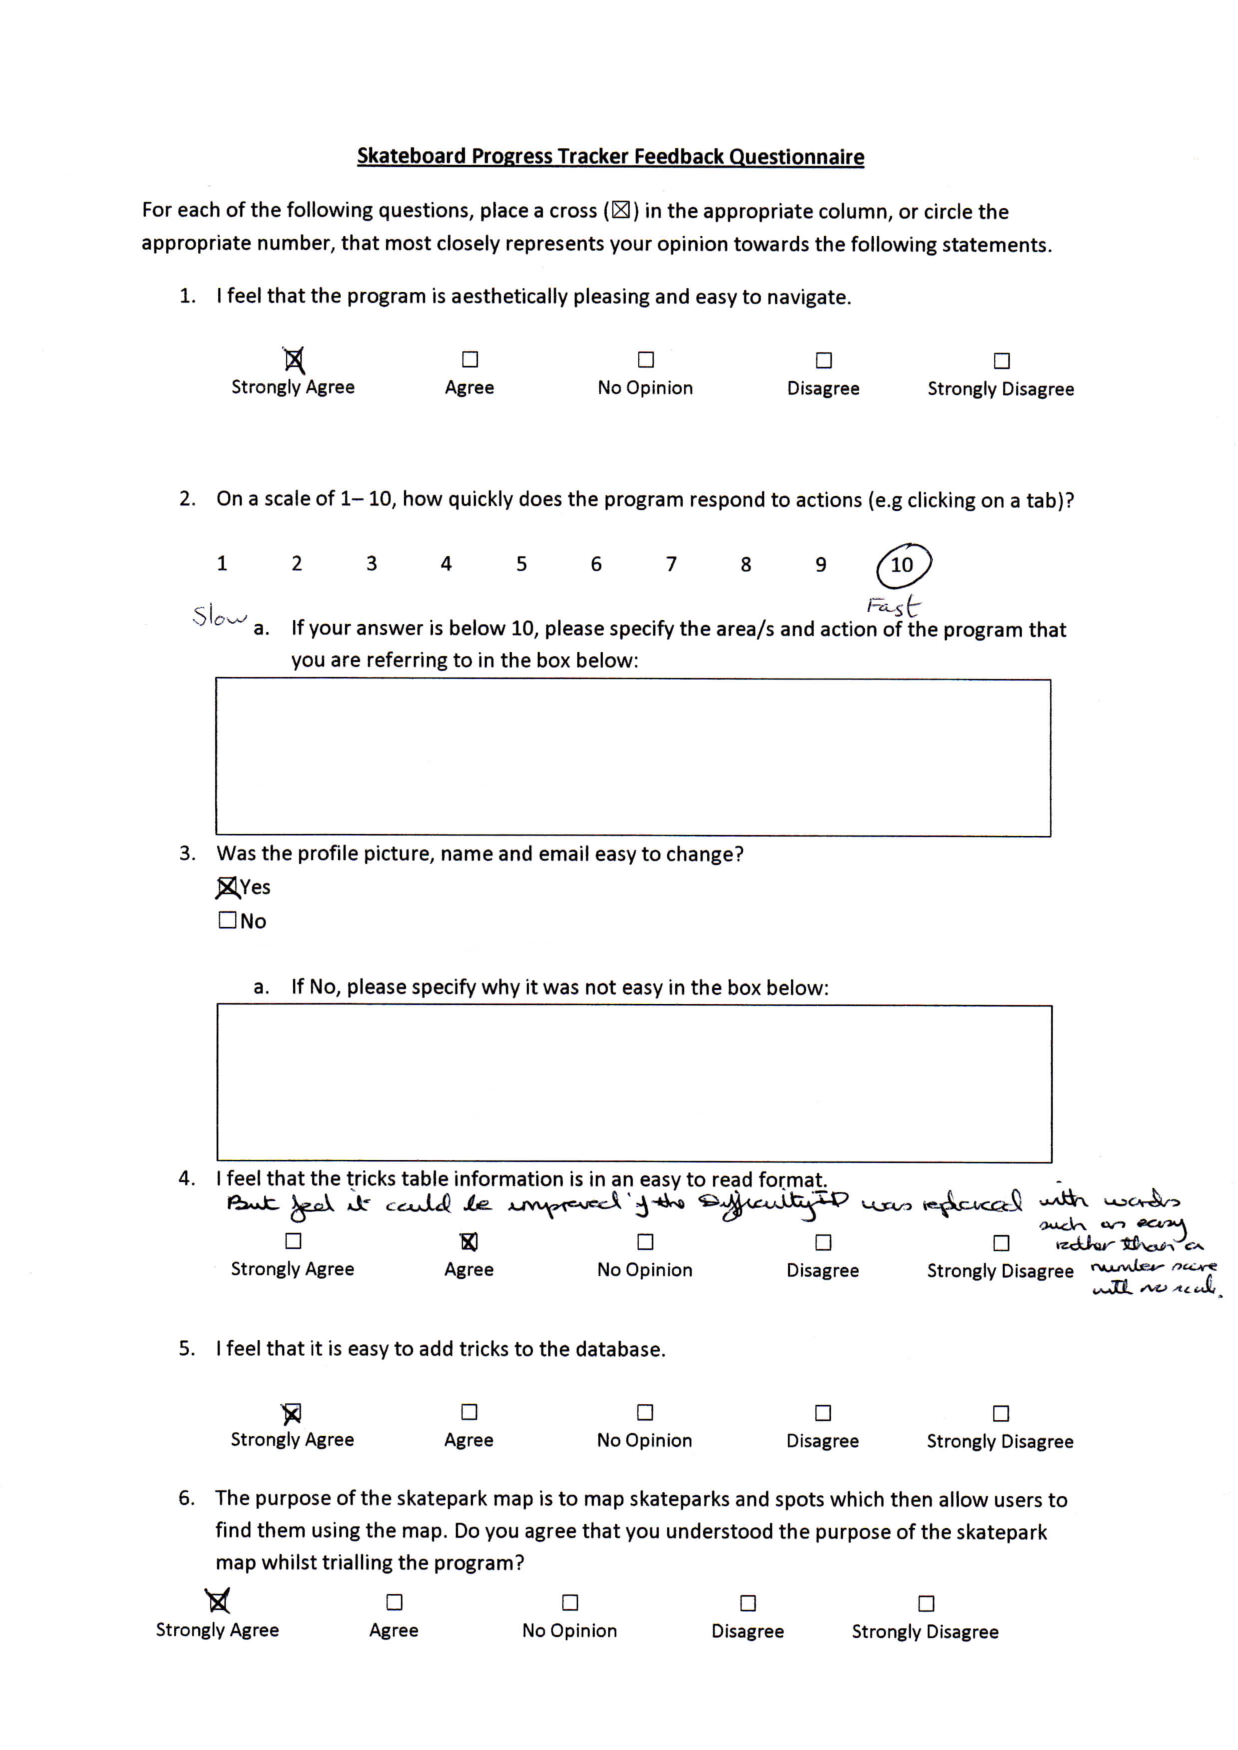
\includegraphics[width=\textwidth]{./Evaluation/images/SueFeedback1.pdf}
    \caption{Sue Feedback Part 1} \label{fig:SueFeedback1}
\end{figure}

\begin{figure}[H]
    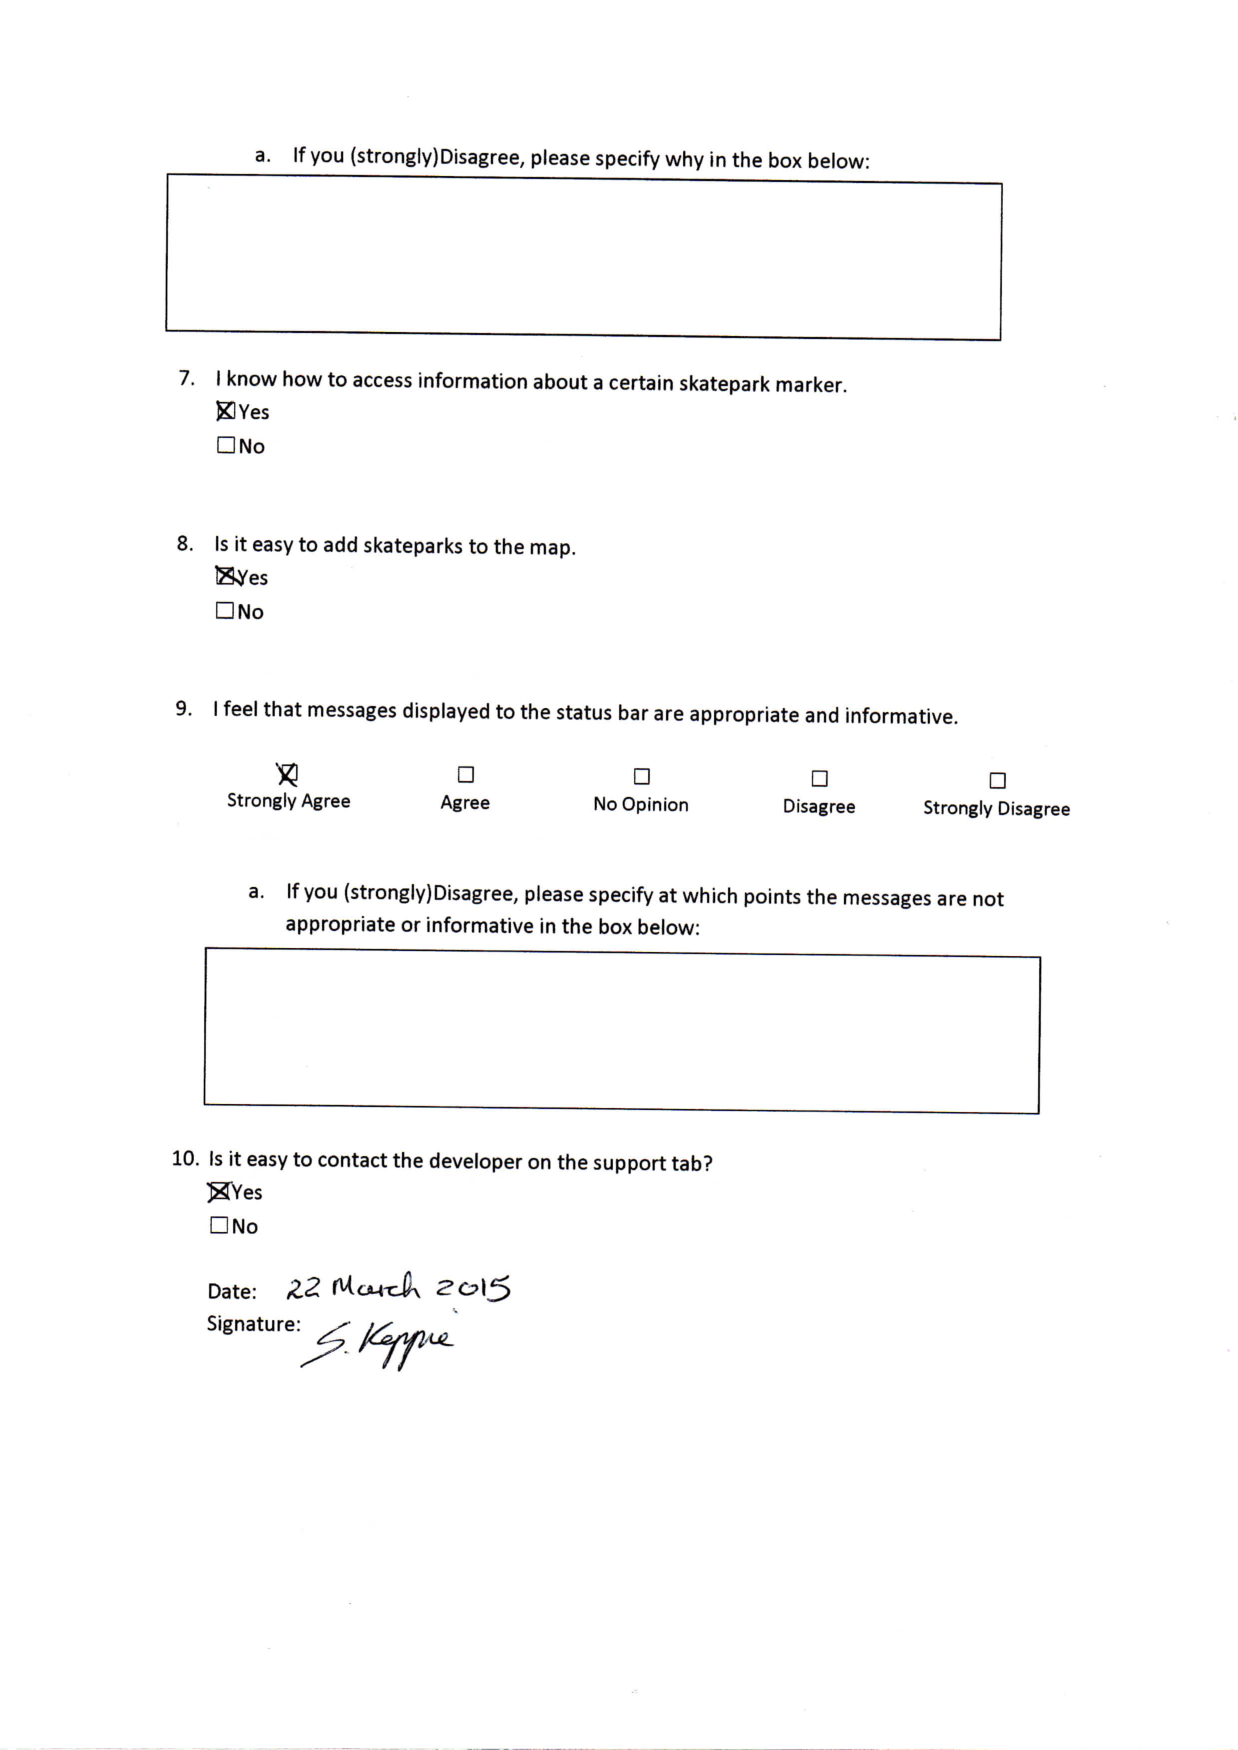
\includegraphics[width=\textwidth]{./Evaluation/images/SueFeedback2.pdf}
    \caption{Sue Feedback Part 2} \label{fig:SueFeedback2}
\end{figure}



\subsection{Graphs}

\subsection{Written Statements}
